
%(BEGIN_QUESTION)
% Copyright 2013, Tony R. Kuphaldt, released under the Creative Commons Attribution License (v 1.0)
% This means you may do almost anything with this work of mine, so long as you give me proper credit

Examine this process trend showing the PV, SP, and Output of a loop controller:

$$\includegraphics[width=15.5cm]{i02636x01.eps}$$

Based on what you see here, determine the following:

\begin{itemize}
\item{} Whether this is an open-loop or a closed-loop response
\item{} Whether the controller is (or needs to be) {\it direct-acting} or {\it reverse-acting}
\item{} If possible, identify any problems with the field instrumentation
\item{} If possible, identify any problems with the controller PID tuning
\item{} Qualitatively identify the kind of PID tuning we will need for robust control
\end{itemize}

\underbar{file i02636}
%(END_QUESTION)





%(BEGIN_ANSWER)

This is a {\it closed-loop test}, based on the fact the output signal responds dynamically to the changing process variable, as well as to the step-change in setpoint.

\vskip 10pt

This is a {\it reverse-acting} controller: the output ramps up whenever the PV is below SP, and the output ramps down whenever the PV is above SP.

\vskip 10pt

This loop definitely has hysteresis in the final control element (e.g. sticky valve), because this trend is a classic {\it slip-stick cycle} in a self-regulating process: the PV exhibits a square-wave shape while the output ramps up and down like a sawtooth wave.

\vskip 10pt

There probably isn't anything wrong with the controller's tuning, and no tuning adjustments will fundamentally address the problem of valve stiction.  

\vskip 10pt

The process appears to be self-regulating with a fast response time (note how quickly the PV settles at a new value following each ``slip'' of the control valve), which means it should control very well with aggressive integral action.  However, final control element hysteresis is the bane of integral action, as it causes repeated reset windup as we see here.

%(END_ANSWER)





%(BEGIN_NOTES)


%INDEX% Process troubleshooting: diagnosing problem via trend recording

%(END_NOTES)


